%% Template originaly created by Karol Kozioł (mail@karol-koziol.net) and modified for ShareLaTeX use

\documentclass[a4paper,11pt]{article}

\usepackage[T1]{fontenc}
\usepackage[utf8]{inputenc}
\usepackage{graphicx}
\usepackage{xcolor}
\renewcommand\familydefault{\rmdefault}
\usepackage{tgheros}

\usepackage{amsmath,amssymb,amsthm,textcomp}
\usepackage{enumerate}
\usepackage{multicol}
\usepackage{tikz}
\usepackage[utf8]{vietnam}
\usepackage[unicode]{hyperref}

\usepackage{geometry}
\geometry{total={210mm,297mm},
left=25mm,right=25mm,%
bindingoffset=0mm, top=22mm,bottom=25mm}

\linespread{1.3}

\newcommand{\linia}{\rule{\linewidth}{0.5pt}}

% custom theorems if needed
\newtheoremstyle{mytheor}
    {1ex}{1ex}{\normalfont}{0pt}{\scshape}{.}{1ex}
    {{\thmname{#1 }}{\thmnumber{#2}}{\thmnote{ (#3)}}}

\theoremstyle{mytheor}
\newtheorem{defi}{Definition}

% my own titles
\makeatletter
\renewcommand{\maketitle}{
\begin{center}
\vspace{2ex}
{\huge \textsc{\@title}}
\vspace{1ex}
\\
\linia\\
\@author \hfill \@date
\vspace{4ex}
\end{center}
}
\makeatother
%%%

% custom footers and headers
\usepackage{fancyhdr}
\setlength{\headheight}{20pt}
\pagestyle{fancy}
\fancyhead{} % clear all header fields
\fancyhead[L]{
 \begin{tabular}{rl}
    \begin{picture}(15,10)(0,0)
    \put(0,-8){
\includegraphics[width=8mm, height=8mm]{hcmut.png}}
    %\put(0,-8){\epsfig{width=10mm,figure=hcmut.eps}}
   \end{picture}&
	%
\includegraphics[width=8mm, height=8mm]{hcmut.png} & %
	\begin{tabular}{l}
		\textbf{\bf \ttfamily Ho Chi Minh City, University of Technology}\\
		\textbf{\bf \ttfamily Department of Computer Science and Engineer}
	\end{tabular} 	
 \end{tabular}
}
\fancyhead[R]{
	\begin{tabular}{l}
		\tiny \bf \\
		\tiny \bf 
	\end{tabular}  }
\fancyfoot{} % clear all footer fields
\fancyfoot[L]{\scriptsize \ttfamily Application Based Internet of Things}
\rfoot{Trang \thepage}
\renewcommand{\headrulewidth}{0.2pt}
\renewcommand{\footrulewidth}{0.2pt}
%



% code listing settings
\usepackage{listings}
\lstset{
    language=Python,
    basicstyle=\ttfamily\small,
    aboveskip={1.0\baselineskip},
    belowskip={1.0\baselineskip},
    columns=fixed,
    extendedchars=true,
    breaklines=true,
    tabsize=4,
    prebreak=\raisebox{0ex}[0ex][0ex]{\ensuremath{\hookleftarrow}},
    frame=lines,
    showtabs=false,
    showspaces=false,
    showstringspaces=false,
    keywordstyle=\color[rgb]{0.627,0.126,0.941},
    commentstyle=\color[rgb]{0.133,0.545,0.133},
    stringstyle=\color[rgb]{01,0,0},
    numbers=left,
    numberstyle=\small,
    stepnumber=1,
    numbersep=10pt,
    captionpos=t,
    escapeinside={\%*}{*)}
}

%%%----------%%%----------%%%----------%%%----------%%%

\begin{document}

\begin{titlepage}
\begin{center}
HO CHI MINH CITY, UNIVERSITY OF TECHNOLOGY \\
DEPARTMENT OF COMPUTER SCIENCE AND ENGINEER
\end{center}

\vspace{1cm}

\begin{figure}[h!]
\begin{center}

\includegraphics[width=3cm]{hcmut.png}
\end{center}
\end{figure}

\vspace{2cm}


\begin{center}
\begin{tabular}{c}
%\multicolumn{1}{c}{\textbf{{\Large BÁO CÁO BÀI TẬP LỚN}}}
\multicolumn{1}{c}{\textbf{{\Large Application Based Internet of Things Report }}}\\
\multicolumn{1}{c}{\textbf{{\Large LAB2B}}}


~~\\

\\
\multicolumn{1}{l}{\textbf{{\Large}}}\\
\\
\textbf{{\Large}}\\

\\
\\

\end{tabular}
\end{center}

\vspace{3cm}

\begin{table}[h]
\begin{tabular}{rrl}
\hspace{5.1cm} 
&\textit{Student: } & Hoang Tran Viet Long\\
&\textit{Student's ID: } & 1652350 \\

\end{tabular}
\end{table}
\vspace{3cm}
\begin{center}
{\footnotesize HỒ CHÍ MINH CITY}
\end{center}
\end{titlepage}

%\thispagestyle{empty}
\renewcommand{\contentsname}{Content}
\newpage
\vspace{1cm}
\tableofcontents
\newpage

\section{Introduction}

In this second LAB, students are proposed to create a simple dashboard using Unity 3D editor.
Basically, the dashboard has 2 screens (GUIs), as depicted following:

\begin{center}
    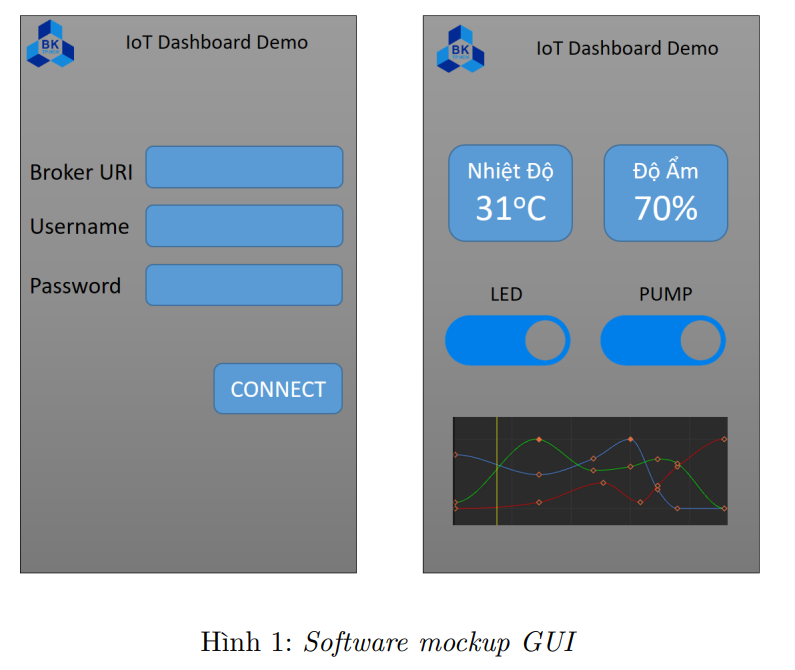
\includegraphics[width=1\textwidth]{Pic1.png}\\
\end{center}

The source code of the second LAB is also required to publish in your GitHub. The details
are described in the next section of this report.

\section{Requirement}

\subsection{Screen 1}

There are 3 input fields, including the broker of the server, username and password. The values of these fields can be set by default (in the design phase, by setting the text property of the input component).\\

When the CONNECT button is pressed, the app will connect to the server. If there is an error, a simple textview can be used to display this error. Otherwise, the second UI is launched.\\

The testing account for this app \textbf{bkiot} and \textbf{12345678} for the username and password. The broker URI is \textbf{mqttserver.tk}. The default port is \textbf{1883}.

\subsection{Screen 2}
The app needs to subscribe to the following topic
\begin{center}
    \textbf{/bkiot/STUDENT\_ID/status}
\end{center}
in order to receive the current values of sensors (e.g. temperature and humidity) and update
these values on textviews. Students can change the information according to their use cases.
However, at least 2 different information of the sensors are required.\\

Two toggle buttons are required to control two different devices (e.g. a simple LED or a
PUMP). When the button is clicked, the data is published to
\begin{center}
    \textbf{/bkiot/STUDENT\_ID/led}
\end{center}
for the LED and
\begin{center}
    \textbf{/bkiot/STUDENT\_ID/pump}
\end{center}
for the PUMP.\\

The data for each button is a json string, described as follow:
\begin{itemize}
    \item {\{"device":"LED","status":"ON"\}}
    \item {\{"device":"PUMP","status":"OFF"\}}
\end{itemize}

\subsection{Advance UI elements}
The end of the second is an example of an advance element in Unity3D. It can be a graph, a
gause or a map. This part is the extra point in this lab.

\section{Report}

\subsection{Screen 1}

\begin{center}
    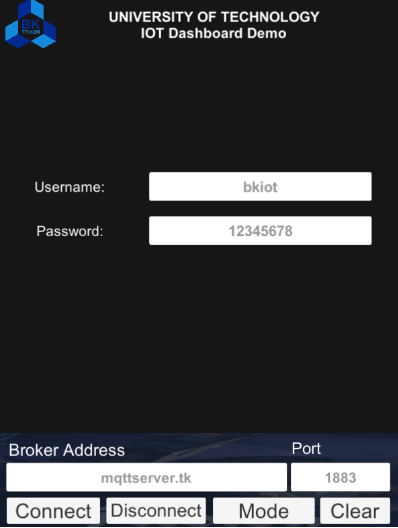
\includegraphics[width=0.5\textwidth]{Scene1.png}\\
\end{center}

\subsection{Screen 2}

\begin{center}
    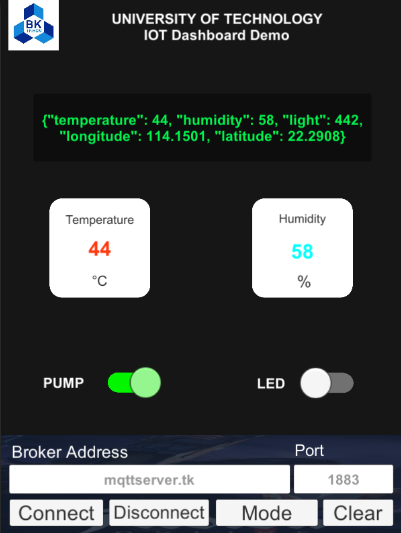
\includegraphics[width=0.5\textwidth]{Scene2.png}\\
\end{center}

\begin{center}
    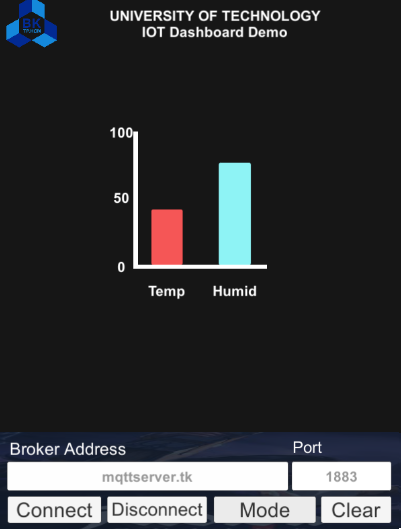
\includegraphics[width=0.5\textwidth]{Scene3.png}\\
\end{center}

\subsection{GitHub link}

\begin{center}
    \textbf{https://github.com/TieuLong98/IOT\_Lab2}
\end{center}
\section{Demo point}
There is a session for live demo. A short meeting for each student will be taken place at google
meet. The schedule for this meeting will be available soon.
\end{document}
